\documentclass[10pt]{article}

%\usepackage{times}
\usepackage{epsfig}
\usepackage{float}
\usepackage{wrapfig}
%\usepackage{oneinchmargins}
\usepackage[margin=1.0in]{geometry}
\usepackage{setspace}
\usepackage{multirow}
\usepackage{graphicx}
\usepackage{paralist}
\usepackage{listings}
%\setlength{\parindent}{0.2in}
%\setlength{\parskip}{2.0pt}

\usepackage{booktabs}
\usepackage[normalem]{ulem}
\usepackage{mathtools}
\usepackage{ragged2e}
\usepackage{rotating}
\usepackage{array}
\usepackage{grffile}
\usepackage{color}
\usepackage{xcolor,colortbl}
\usepackage{chngpage}
\usepackage{enumitem}
\usepackage{amsmath,relsize}
\usepackage[justification=centering]{caption}
\usepackage{paralist}

\renewcommand{\topfraction}{1.00}
\renewcommand{\dbltopfraction}{1.00}
\renewcommand{\bottomfraction}{1.00}
\renewcommand{\textfraction}{0.00}
\renewcommand{\floatpagefraction}{1.00}
\renewcommand{\dblfloatpagefraction}{1.00}

\newcommand{\Forall}{\displaystyle\mathop\mathlarger{\mathlarger{\mathlarger{\forall}}} } 

\title{{Exploring the Parallel Programming Design Space of \\
        Proximate, a Multi-Tile Programmable Accelerator}\\ 
        { \normalsize (CS 758 Project Report)}}
        \author{Vinay Gangadhar and Kai Zhao \\University of Wisconsin-Madison\\{\tt \{vinay, kzhao32\}@cs.wisc.edu}}
\date{}
\begin{document}

\maketitle

%\onehalfspacing
\doublespacing

\begin{abstract} 

The slowing of Moore’s law and Dennard scaling is limiting the performance 
improvements of single core processors. 
Increasing clock frequency any farther will lead to 
high leakage current and infeasible power consumption.
Over the past decade, focus has been shifted to multi-core processors 
to increase throughput by having multiple cores  to target
different types of parallelism - instruction (ILP), data (DLP) and  thread (TLP).
However, even the multi-core processors are not scalable for parallelization beyond a point 
due to Amdahl's law. To address these challenges of rising dark silicon and the end
of Dennard scaling, in recent years architects have turned to heterogeneous architectures 
with special purpose domain specific accelerators (DSAs), for higher performance and energy efficiency.
While providing huge benefits, DSAs are prone to obsoletion due to domain volatility,
have recurring design and verification costs, and have large
area footprints when multiple DSAs are required in a single
device to reap out the benefits of different application acceleration.
To attack such problems of DSAs and multi-core processors, 
while still retaining programmability of general purpose processors and 
efficiency of DSAs, there is an on-going research in Vertical Research Group, University of Wisconsin-Madison
aiming to build a general purpose multi-tile programmable accelerator called Proximate. 

This project focuses on exploring the parallel programming design space
of Proximate, a multi-tile programmable hardware accelerator.
The aim is to investigate the programming interface  of Proximate, the parallel
hardware improvements and in general explore the parallel programs run on proximate.
We have tried to explore a new type of the multi-tile programmable architecture,
its scalability and speedup of such accelerator architecture 
compared to a traditional server class multi-core processors for parallel programs.
In summary, we explored different programming design points in the project and proximate is able to achieve speedups of
50-100x over a traditional server class multi-core processor. We try to analyze this trend over the coarse of this
document by explaining the architecture, programming model and the performance results of proximate. 

\end{abstract}


\section{Introduction}

The end of classical device scaling means that the power per unit area on chip
is rising with each technology generation.  This implies that architectures for
future technology nodes will not be able to power-on all components of the chip
simultaneously, with some estimates being 50\% ``dark silicon'' by
8nm~\cite{isca11:dark-silicon}, which is less than 10 years away.  This trend,
the utilization wall, will curtail expected performance improvements.
Interestingly, much of the core's energy is not expended in the functional
units, but rather in the power-hungry structures needed for
attaining reasonable performance on general purpose workloads.  To exploit this,
architects have in part turned to hardware specialization and
accelerators, which sacrifice generality for efficiency in executing either
specific computations or computations for certain application domains.

Though accelerators hold great promise, with many new accelerator designs
showing significant efficiency and performance gains, the research and 
insights have been fragmented.  Newly proposed accelerators are evaluated 
in their own toolchain, generally with a specific general purpose core, and with 
a set of chosen benchmarks.  Solving this by integrating tens of accelerators 
into a single simulation system and developing compatible compilers 
for them is intractable due to development time.  This means that attaining 
insights into accelerators which transcends specific simulators, core design
points, evaluation metrics and applications is extremely difficult.
This limitation hinders our ability to understand the future of acceleration 
in terms of their behavior, design and use.
%benefit, and how can we do it?

%insights into how the applications and choice of 
%general-purpose core affects what is the best accelerator 
%to apply is very difficult.  Also, this lack of information hinders our ability
%to see what are the future opportunities for acceleration: where can we get more
%benefit, and how can we do it?

Going forward, the architecture community needs a methodology for modeling
acceleration which is detailed and accurate, yet simple and abstract, to help
unify and improve the current understanding.  With such a
tool, we can begin to address the biggest challenges of acceleration:  First,
we must understand where the biggest benefits of acceleration could come from,
and what are the biggest limitations, so we can best focus our efforts on
problems which will push the limits of their effectiveness (\emph{Finding
Accelerator Limits/Opportunities}).  Second, we need a strategy for designing
accelerators which can explore a broad range of the possible space in a short
amount of time (\emph{Effective Practices for Accelerator Design}).  Finally,
we need practical and flexible ways to employ multiple accelerators at
runtime so that the promises of accelerators can be achieved in a
wide variety of domains (\emph{Enabling Practical Multi-Acceleration}).

In pursuit of these challenges, this dissertation proposes 
a novel abstraction called the Transformable
Dependence Graph (TDG), which can model certain important forms of acceleration.  
It is designed to accurately capture interactions between the accelerator, general
purpose core, and application at sub-instruction granularity.   The core idea is to
represent the program’s execution trace as a dependence graph of
micro-architectural events, and to perform transformations on this
representation to model various forms of acceleration.  This concept is based
on the dependence-graph of Fields \emph{et
al.}~\cite{fields:isca01,Fields:2002:SMP:545215.545222}, and our contribution is
in showing how graph transformations can model acceleration.

\subsection{Completed Work}
Completed work has shown that our model and implementation is accurate in
capturing both the out-of-order execution of processors, as well as the
transformation from OOO dependence-graph trace to model four different classes
of accelerators.  Our results have shown that, using the dependence-graph model, we can
achieve an average error of less than 15\% in both performance and energy
reduction for all classes of accelerators we target. In general, there are
certain accelerator classes which can be modeled accurately, discussed in
detail in Section~\ref{sec:scope}~(Page~\pageref{sec:scope}).  
The flexibility, accuracy, and high-abstraction of the TDG is useful for 
solving a variety of problems beyond just modeling, 
and forms the basis for the proposed research.  

%The TDG can be used for purposes beyond modeling, and this proposed
%work is described next.

%Using the TDG we have three primary research directions.  First, we
%aim to understand what are the limitations and opportunities with
%currently proposed accelerators.  By formalizing architectural
%optimizations as graph transformations, we can quickly explore the
%potential of an architecture.  Second, we can use the TDG to help design
%new accelerators.  By finding applications which are not exploited by
%current accelerators, we can use this insight to develop next generation
%accelerators which are complementary to existing designs.  Also, the
%abstract nature of the TDG enables rapid design space exploration, and
%by associating transformations with units of hardware, we may be able to
%partially to fully automate this process.  Finally,  if multiple
%accelerators can provide high benefits, then we will need practical ways
%of scheduling them.  We will explore how to use dynamic execution
%information along with performance/efficiency goals to schedule
%accelerators.

\subsection{Summary of Proposed Work}

%By employing the TDG as an efficient modeling tool, my proposed work addresses
%the aforementioned accelerator challenges.
Figure~\ref{fig:proposed-work-overview} gives a high-level overview of each
proposed work compared to the current approaches for each problem, 
and they are outlined below.

\begin{figure}
\vspace{-.2in}
\begin{adjustwidth}{-0.3in}{-0.3in}
  \begin{center}
    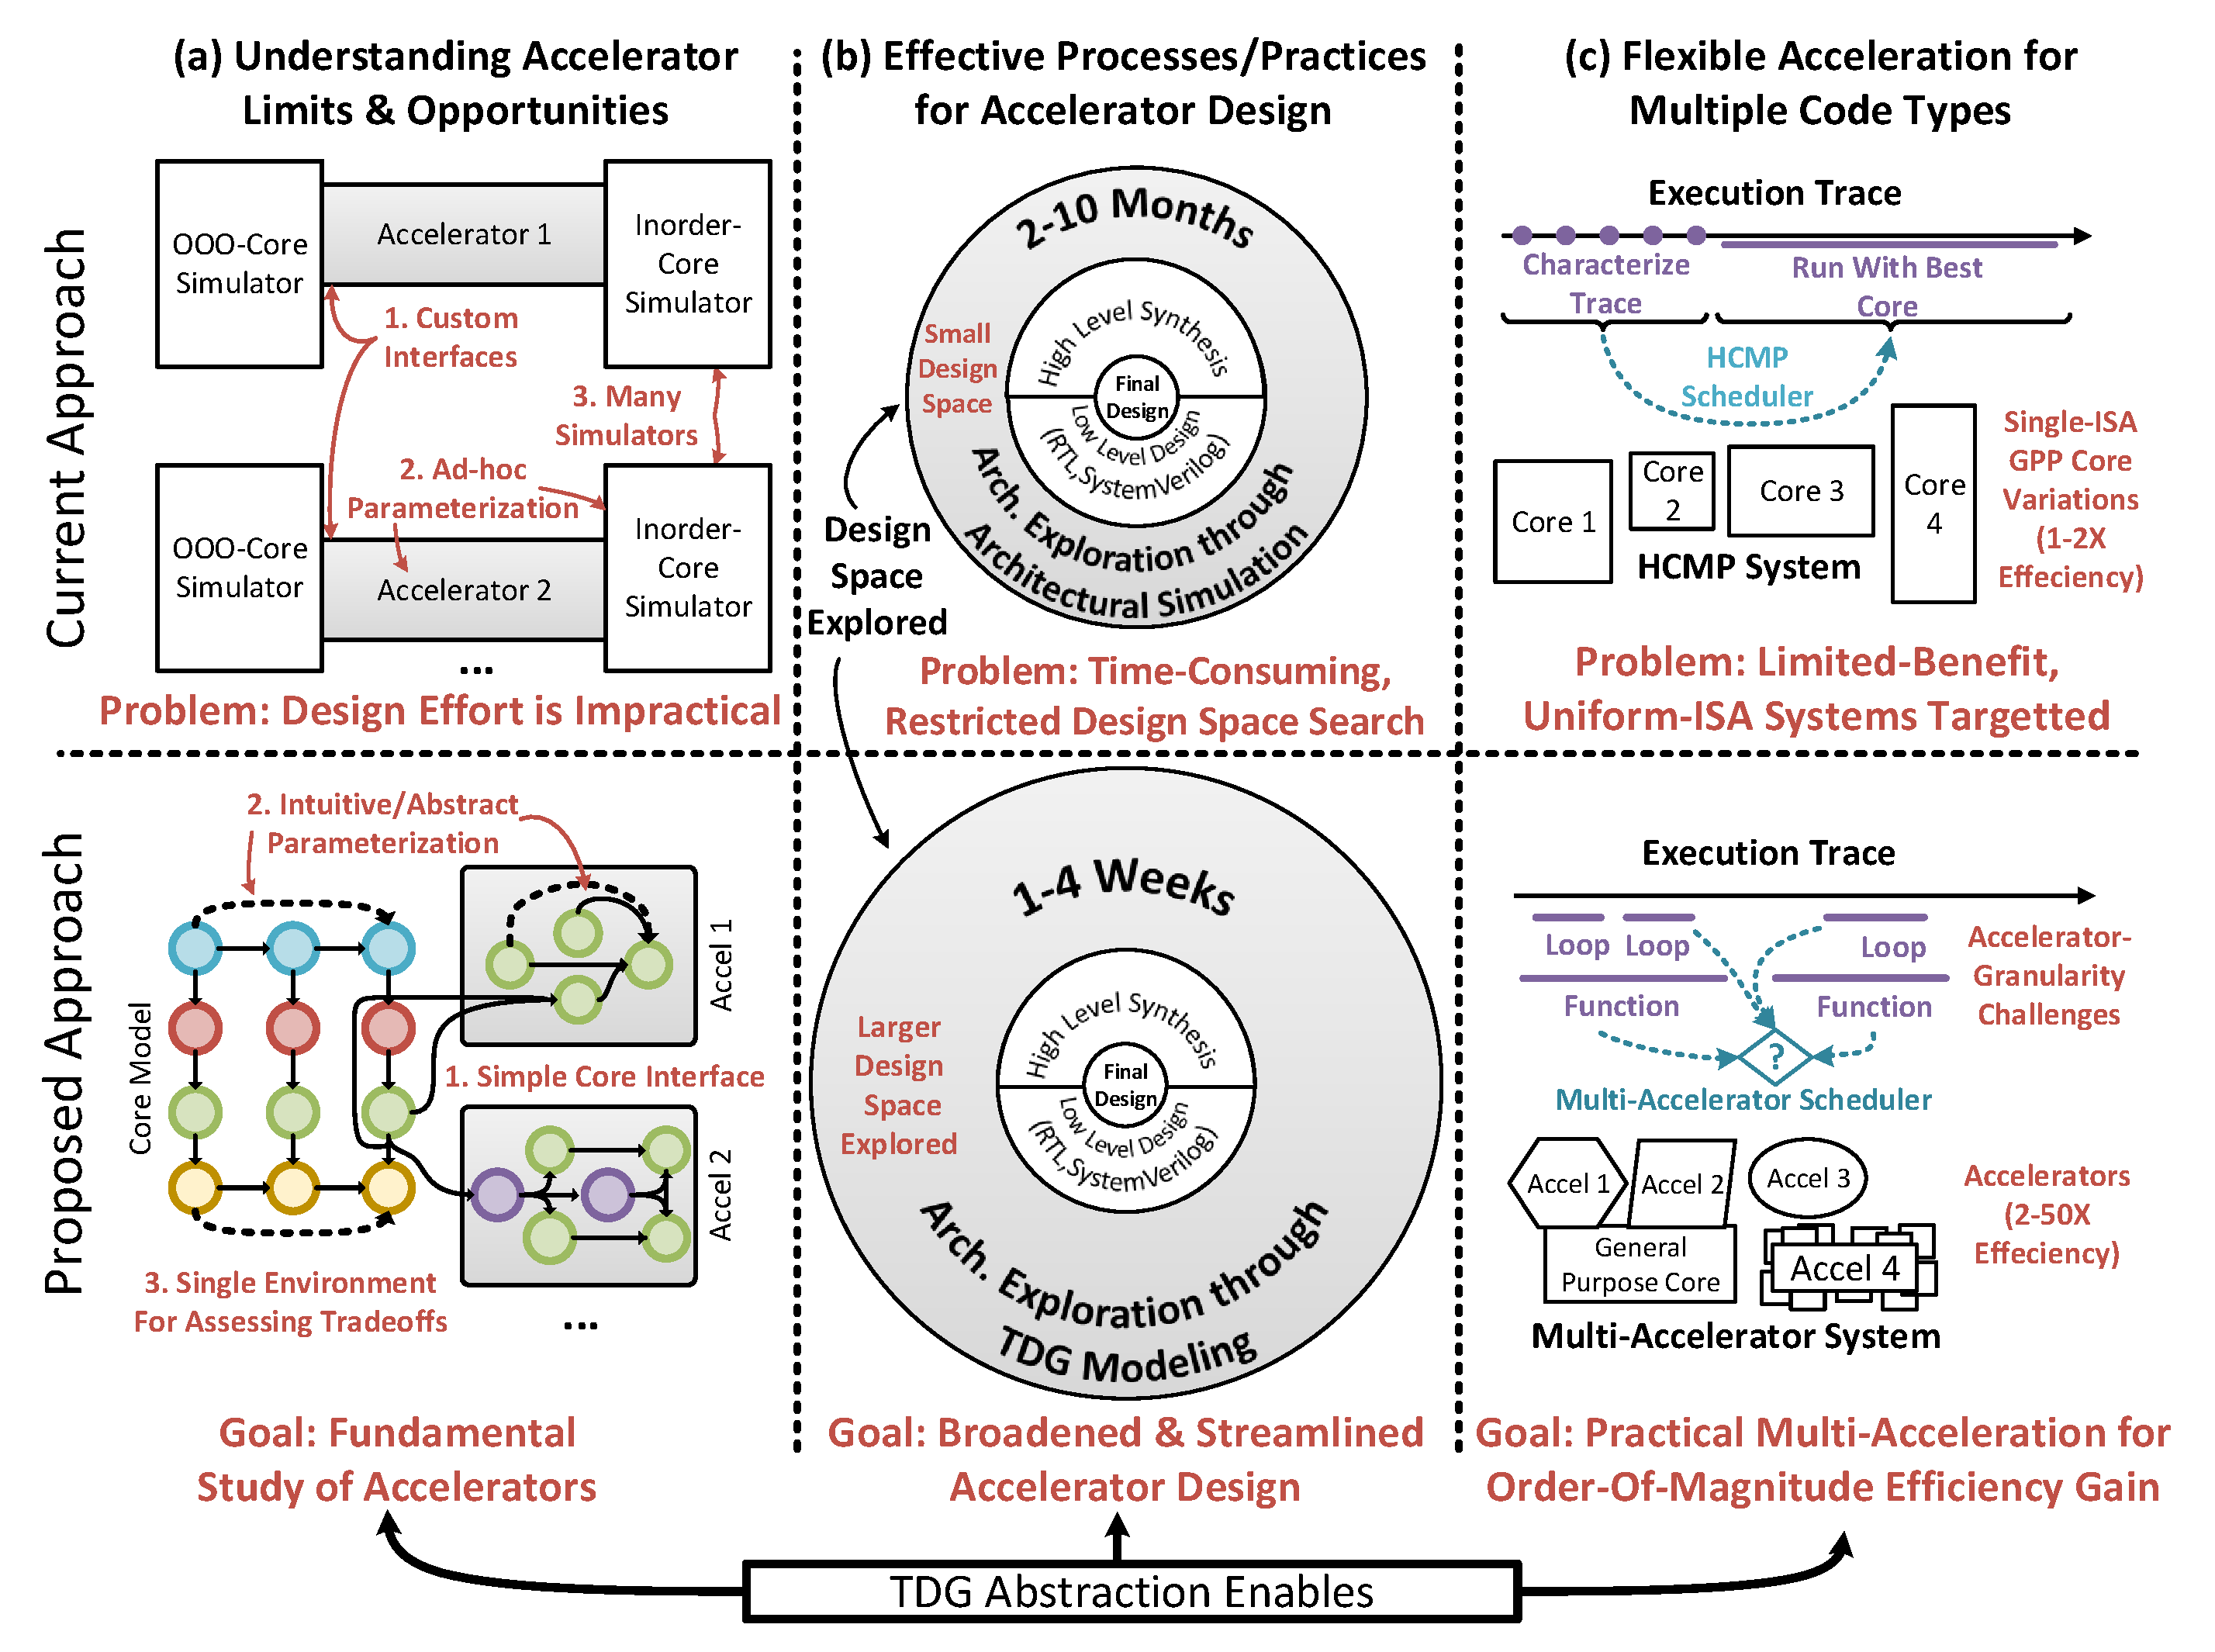
\includegraphics[width=1.0\linewidth]{figs/proposed-work.pdf}
  \end{center}
\vspace{-0.2in}
  \caption{Summary of proposed work as compared with current best techniques.}
  \label{fig:proposed-work-overview}
\vspace{-0.05in}
\end{adjustwidth}
\end{figure}


\begin{itemize} \item \textbf{Limits and Opportunities of Acceleration:} For the
future of acceleration, it is important both to understand the fundamental
limitations of accelerators, as well as to know where the largest benefits can
come from.  We can better understand accelerators by modeling hypothetical
designs which break current limitations, and observing their new behavior.
Current approaches using simulators would be too tedious because they require
ad-hoc accelerator implementation and integration with multiple simulators. The
proposed approach employs the TDG to simplify modeling and unite the modeling
of accelerators under a common framework, making the study of their nature
consistent and practical.  This work's goal is to uncover the fundamental
limitations of accelerators, to show what are the most important challenges for
future accelerator architects.


\item \textbf{Effective Processes/Practices for Accelerator Design:} Existing
accelerator design strategies are ineffective because they rely on tedious
simulator modeling, consider accelerators in isolation, and inappropriately bin
applications to accelerator designs.  Overall, they are able to cover less of
the design space, and require more design time.  To address this, this research
proposes an accelerator design strategy which leverages the TDG.  Primarily, it
presents a higher level of abstraction, both broadening the explored design
space while hastening the process.  The unified framework makes it simple to
compare with existing accelerators during the design-space exploration, which
can help prune the design space quickly.  Also, many TDG models can be used
together to find the regions with the biggest potential for new accelerators,
giving insight to architects without the need to bin accelerators.  The
research so far shows how to use the TDG to help design an accelerator for
nested loops, a contribution on its own.

\item \textbf{Enabling Flexible/Practical Multi-Acceleration:} 
By employing multiple accelerators in a single system, it is possible to achieve
flexible efficiency for a variety of code types.  Current approaches lack the
ability to target systems more general than uniform-ISA heterogeneous architectures.
To attain the benefits of multi-acceleration, it is
necessary to partition regions of applications onto the most beneficial
accelerator.  This decision can be complicated, because
accelerators are only legal on different granularities of code.
Also, certain accelerators can have serious drawbacks if applied on the wrong
application regions.  The proposed research is to explore static
and dynamic mechanisms, including intuition-guided static approaches, 
compiler-generated TDG-based prediction, multi-granularity sampling techniques, 
and machine-learning based performance/energy models.  

\end{itemize}

\subsection{Relation to My Previous Work}

The inspiration for this dissertation topic stems from my previous work in creating
a unifying general framework for spatial architecture scheduling~\cite{ILP_Sched},
which received a distinguished paper award.
That work leveraged a mathematical theory, namely integer linear programming,
to create abstractions which enabled the modeling of scheduling 
constraints and characteristics common across a wide variety of architectures.
This work in turn inspired us to co-author a synthesis lecture on the use of
optimization and mathematical modeling in 
computer architecture~\cite{DBLP:series/synthesis/2013Sankaralingam}.

My previous work is related to this dissertation work in two ways.  First, the
principles of creating a general framework, using higher-level abstractions and
mathematical modeling of architectural phenomenon are common to both.  Second,
and more concretely, the instruction scheduling techniques developed are
modified and employed for some newly developed accelerators we consider.

\subsection{Document Overview}

Section~\ref{sec:tdg} describes completed work in using the TDG to model various forms of
acceleration, in terms of modeling and validation.  The next three sections
describe the proposed work: Section~\ref{sec:limits} for studying the limits
and opportunities, Section~\ref{sec:design} for using the TDG to aid the design
of new accelerators and Section~\ref{sec:multi-acc} for enabling practical
multi-acceleration.  Each section of proposed work contains a \emph{motivation}
section, a \emph{research approach} section to explain how we address the problem,
a \emph{preliminary results} section, a \emph{proposed work} section 
which overviews the remaining work to be done, and ends with \emph{related work}.
Section~\ref{sec:summary} summarizes the work, 
Section~\ref{sec:deliverables} outlines deliverables,
and Section~\ref{sec:timeline} describes the proposed dissertation schedule.


\if 0
Accelerators are units of hardware which specialize aspects of a general 
purpose processor's execution to improve performance and/or efficiency.  
They firstly do this by exploiting particular aspects of a target application domain.
A popular example is SIMD, which specializes for data-parallel computation, and
another is Coarse Grain Reconfigurable Architectures (CGRAs),
 which specialize for computation pattern re-use.  The way that accelerators
rely on applications for certain properties is what we call \emph{accelerator-application}
interaction.

In addition to exploiting properties of applications, accelerators also use
specific hardware techniques to reduce the overheads
of a general purpose processor.  SIMD processors have parallel datapaths, and
reduce instruction count, and CGRAs employ reconfigurable datapaths.
The strategies by which accelerator's specialize the general purpose core is what
we call the \emph{accelerator-core} interaction.
Table~\ref{tab:overview} lists the application properties that four prominent
accelerator classes exploit, and the ways by which they specialize the
core's execution.
\fi







%architecture~\cite{smith:dae}, I propose a decoupled architecture
%that avoids disruptive changes to existing microarchitecture to
%dynamically create custom hardware datapaths.
%Second, I design and implement a compiler that avoids
%disruptive changes to traditional programming model.
%\end{itemize}
%extends makes only small modification to existing archmicroarchitecture 


%Para 5:
%What I specially proposing to do

%Para 6:
%This document is organized as follows.  First, 



\section{Prior Work and Project Proposal} \label{sec:prior}

We build our project on the prior work done on LSSD~\cite{nowatzki2016pushing} (Work done in Vertical Research Group), which includes identification of specialization principles and proposal of the
high-level architecture of the high throughput compute engine (called Softbrain now). Softbrain builds 
upon the LSSD principles and implements the general micro-architectural mechanisms identified in prior work. 
Before explaining the high level organization of Proximate architecture, the five
specialization principles employed to consider this style of accelerator architecture are explained. 
The primary insight 
on coming to the architectural substrate is based on well-understood mechanisms of specialization used in
DSAs. 

\subsection{Specialization Principles}
Broadly, these principles are seen in as a counterpart to the insights from Hameed et al.~\cite{1815968}, in that they describe the sources of inefficiency in a general purpose processor, whereas our findings are oriented around
elucidating the sources of potential efficiency gain from specialization.

\paragraph{Concurrency Specialization}
The concurrency of a workload is the degree to which its operations can be
performed in parallel. This concurrency can be derived from data or thread level parallelism found in the
workloads. Examples of specialization strategies include employing many independent processing elements
with their own controllers, or using a wide vector model with a single controller. The former one is chosen as
baseline architecture having many processing elements with a low-power controller.

\paragraph{Computation Specialization} Computations are individual units of work in an algorithm executed by
functional units (FUs). Specializing computation means creating problem-specific FUs. For instance, a sin
FU would much more efficiently compute the sine function than iterative methods on a general purpose
processor. Specializing computation improves performance and energy by reducing the total work. Most of
the neural network applications employ some commonality in FU types.

\paragraph{Communication Specialization} Communication is the means of transmission of transient values between
the storage and functional units. Specialized communication is simply the instantiation of communication
channels, and potentially buffering, between FUs to ultimately facilitate a faster operand throughput to the
FUs. This reduces power by lessening access to intermediate storage, and potentially area if the alternative is
a general communication network.

\paragraph{Data Reuse Specialization} Data reuse is an algorithmic property where intermediate computed values
are consumed multiple times. The specialization of data reuse means using custom storage structures or
reuse buffers for these temporaries. Specializing reuse benefits performance and power by avoiding the more
expensive access to a larger global memory or register files.

\paragraph{Coordination Specialization} Hardware coordination is the management of multiple hardware units and
their timing to perform work. Instruction sequencing, control flow, interrupts handling and address generation
are all examples of coordination tasks. Specializing it usually involves the creation of small finite state
machines to perform each task. A low-power in-order core or a micro-controller could be used for this
coordination specialization. Based on the this principle, to aim at high concurrency workloads and provide 
the task/data locality to 
programmers, Proximate has lot of  such small in-order cores acting both 
as coordination unit and computation engine to execute irregular workloads. This is based heavily on the 
principle of having many small in-order cores near memory to do the high-throughput computation~\cite{menon2014memory}.

Based on extensions to all the prior work explained above,
we currently have built a vector dataflow programmable accelerator 
called Softbrain that is general purpose  
programmable using a high level hardware 
programming interface (HPI). 
Regular streaming workloads that are mainly 
single threaded showed comparable performance to the 
fixed function implementation of these workloads. 
The current research also aims at having a general purpose 
programmable tiled organization of 
in-order cores which run single threaded fine-grained parallel tasks,
connected to the programmable accelerator (Softbrain) briefed above. 
Together this entire hardware organization targets both 
irregular and regular workloads, and we call 
this combined organization of hardware as Proximate. 
Proximate combines this multi-core tiled architecture with
programmable/specialized accelerator (Softbrain) together into a 
single external PCIE device. Figure~\ref{fig:prx-orig} shows high-level
overview of the current Proximate offload engine. 

\begin{figure}
  \begin{center}
    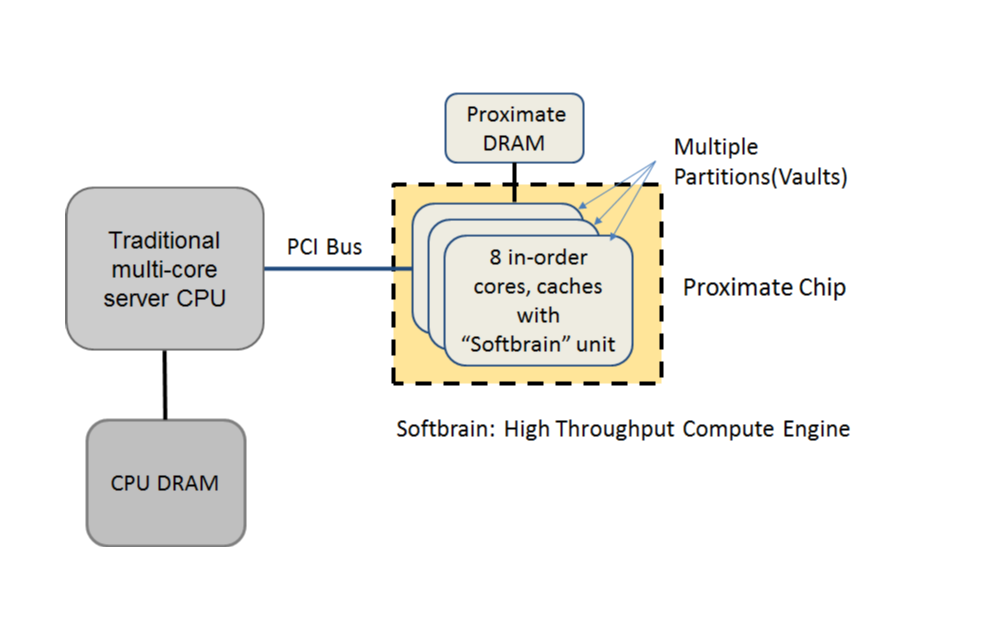
\includegraphics[width=\linewidth]{cs758-figs/prx-orig.png}
  \end{center}
\vspace{-0.9in}
  \caption{Proximate Offload Engine}
  \label{fig:prx-orig}
\vspace{-0.05in}
\end{figure}

Proximate has a 16 compute tiles, 
each compute tile with 8 (RISC-V) in-order cores, 
a programmable/specialized accelerator (softbrain
fabric) for a total of 128 RISC-V inorder cores and 
16 softbrain fabric instances connected to a common 
memory hierarchy. It is programmable using a high-level 
offload API to offload the data, allocate memory on device and 
copy the data to/from the host processor. 


\subsection{Project Proposed}
Since, we exactly cannot have the same hardware model setting as Figure~\ref{fig:prx-orig},
for our project, we have to slightly modify the API as well as the hardware model to suit our experiments.
Figure~\ref{fig:prx} shows the organization of the entire device for our
project purposes. We assume both the host core and the proximate device
to be located in the same shared address space and proximate operates
in a memory mapped region of the shared address space. 
The host core also runs the Proximate parallel programming API and the runtime
is responsible for offloading the tasks at coarser-granularity to a device-specific
task scheduler. This task scheduler is connected to the proximate tiles, with each tile
having group of in-order cores and the high-throughput compute engine, Softbrain. 


\begin{figure*}[h]
  \begin{center}
    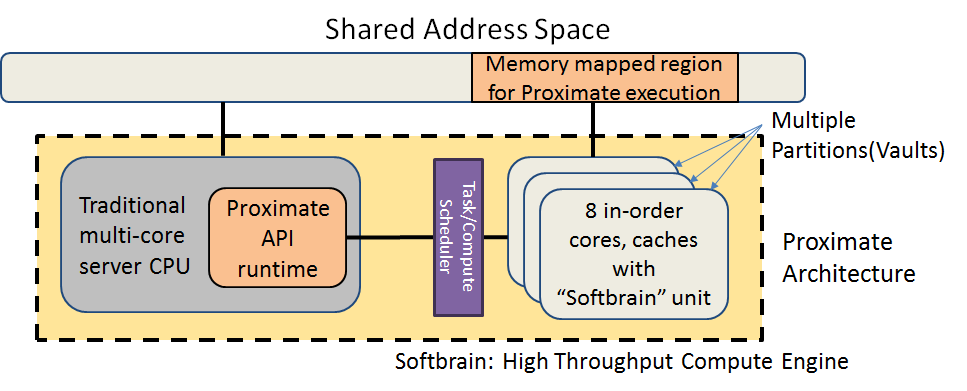
\includegraphics[width=\linewidth]{cs758-figs/proj.png}
  \end{center}
\vspace{-0.2in}
  \caption{Proximate Architecture in Our Project Setting}
  \label{fig:prx}
\vspace{-0.05in}
\end{figure*}

This project aims to parallelize some of the 
single-threaded regular HPC workloads and 
irregular workloads on Proximate architecture 
and evaluate performance and bandwidth 
limitations compared to a server class chip 
like 64-core Xeon Phi Knights landing.
We start this by converting all the single-threaded workloads
to the parallel versions of pthreads and OpenMP. Th idea behind this
is to get the data from real hardware as well as see the scalability of these parallel workloads.
We then implement the proximate versions of the parallel programs and evaluate the performance
w.r.t to the best configuration of pthread run on Xeon-Phi. 




\section{Motivation} \label{sec:motiv}

As we mentioned earlier, general purpose cores are highly inefficient 
and are optimized for single thread workloads only. They have very low energy efficiency
for server workloads mainly due to high-frequency, deep  pipelines, speculation
and explicit memory/register based communication~\cite{gpp_innef}.
Even the new heterogeneous offload engines like GPUs,FPGAs and ASICs face either 
programming or power-area challenges. So, this motivates us to
invent new heterogeneous offload engines which - i) achieves better scalability
and higher performance per watt, ii) have flexible programmer abstraction and
iii) able to target different program behaviors in the core regions -- both regular and irregular.  

With such requirements, this section tries to motivate why this type of architecture and programming abstraction
is needed for Proximate, and what are some of the insights and mechanisms needed to arrive 
at such architecture for current parallel workloads. 

\subsection{Insights}
The main insight for parallelization in Proximate is that - it
is reasonable to presume that programmer can reason about the
data/task locality of the kernel. Programmer managed data sharding
and task/data co-location is fairly straight forward for several server class
workloads. 
By co-locating the data and task you would reduce the access latency and 
achieve higher memory or cache bandwidth. 

The other insight we had was, each program or application can have multiple phases
during the program execution~\cite{nowatzki2016analyzing}. So, your
parallel hardware must be able to recognize such phases and offload the kernel to
corresponding hardware in a heterogeneous environment. Program regions generally tend to 
exhibit two main behaviors - i) Irregular data access pattern with low ILP and
ii) Regular data access patterns with high DLP. So, the architecture executing such programs need to
accelerate both these regions and the insight is to execute both these phases in proximate.
The final insight is that, since regular workloads are memory streaming workloads, the architecture needs
to support high bandwidth memory hierarchy and should be able to provide sufficient memory bytes in less number of cycles. 

\subsection{Mechanisms to Exploit Insights}

We now explain some of the mechanisms we have come up with to exploit the 
insights described above. 
\paragraph{Programmer Control Data/Task Locality}
The high level question one has to ask in how to give the programmers control
of data and task locality within proximate cores. We answer this
in Proximate by providing a flexible programming model to enable the 
programmer managed data sharding and task/data co-location. 
Figure~\ref{fig:prog-overview} shows the programmer's view of the architecture, 
and the vault abstraction proximate provides. Each vault is group of cores
and a predetermined slice of virtual address spaces, exposed during task offloading 
and memory allocation. 

\begin{figure}
  \begin{center}
    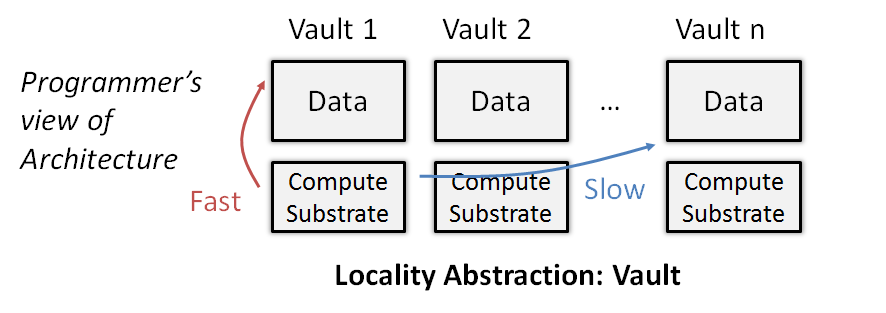
\includegraphics[width=\linewidth]{cs758-figs/prog-abs.png}
  \end{center}
\vspace{-0.2in}
  \caption{Programmer Abstraction of the Architecture}
  \label{fig:prog-overview}
\vspace{-0.05in}
\end{figure}


The locality abstraction for programmers is given by the vault. Each vault, 
has an address partition (data) and the compute substrate to work or offload task
on that address partition. There is a latency penalty if each compute substrate does an 
out-of-vault access to access data not in its address partition. By giving this abstraction to 
programmer, he/she can manage the data sharding explicitly and reason about the data/task locality.

\paragraph{Program Regions and Memory Bandwidth Requirement}To satisfy the high bandwidth demand and memory requirement, Proximate has address partitioned
per-vault caches. Proximate has simple in-order cores to target program regions exhibiting irregular data access patterns with low ILP. 
It has a high throughput compute engine (Softbrain) to target program regions exhibiting regular data access patterns with high DLP.

\section{Proximate Architecture and Programming Overview} \label{sec:arch}



\subsection{Architecture Overview}
In this section we first desribe the high-level architecture 
overview of the general purpose programmable accelerator - Porximate. 





\section{Proximate Programming Interface and API} \label{sec:prog}

This section gives an overview of Proximate programming interface or API
and how one would program the entire application using proximate API.
And then we will describe the task based queuing model we have implemented
for proximate to scheduled tasks for in-order cores as well as Softbrain.

\subsection{Proximate API}
At a high-level Proximate API is very much similar to any task based
API like Cilk~\cite{leiserson2010cilk++} or TBB~\cite{pheatt2008intel}.
The only difference is the way memory gets allocated in each of the
vault and the data sharding part where the programmer has to explicitly do a 
copy of the data structures to each of these vault allocated structures. 

\paragraph{Kernel Context and Loading}

\begin{figure}[h]
  \begin{center}
    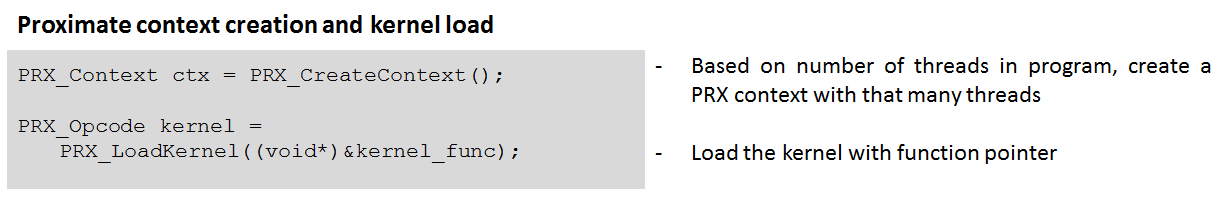
\includegraphics[width=\linewidth]{cs758-figs/api-alloc.png}
  \end{center}
\vspace{-0.2in}
  \caption{API for Context Creation and Kernel Loading}
  \label{fig:api-kernel}
\vspace{-0.05in}
\end{figure}

Figure~\ref{fig:api-kernel} shows the code snippet for Kernel creation
and loading the kernel to device memory location. 
This API can be used by the programmer to register a function/kernel, 
located in the host address space, with the Proximate library. 
The input argument is the function pointer to the kernel in the host virtual address space.
The return value is the index of the page in the Proximate “code Region”.   

\paragraph{Memory Allocation}
The next API is for the memory management on Proximate memory mapped region. 

\begin{figure}[h]
  \begin{center}
    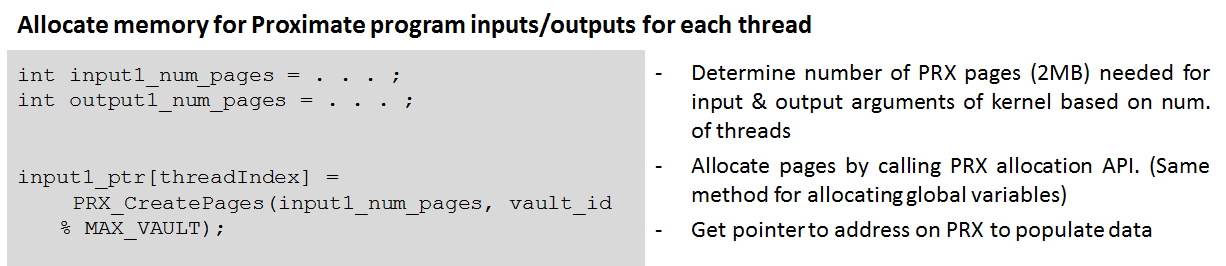
\includegraphics[width=\linewidth]{cs758-figs/api-copy.png}
  \end{center}
\vspace{-0.2in}
  \caption{API for Input Arguments Memory Allocation}
  \label{fig:api-mem}
\vspace{-0.05in}
\end{figure}

\begin{figure}
  \begin{center}
    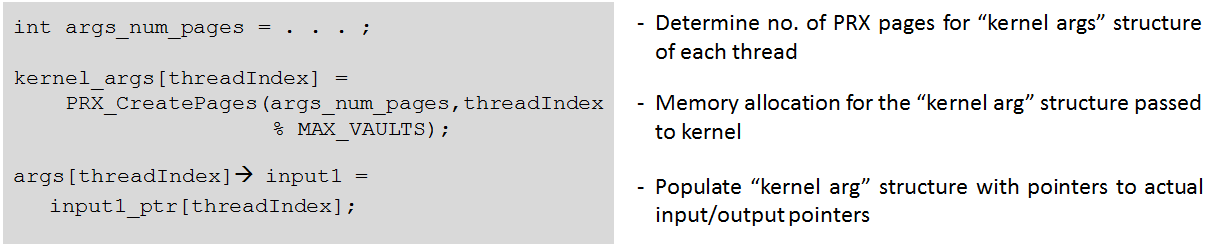
\includegraphics[width=\linewidth]{cs758-figs/api-arg.png}
  \end{center}
\vspace{-0.2in}
  \caption{API for Kernel Argument Structure Allocation}
  \label{fig:api-arg}
\vspace{-0.05in}
\end{figure}

Figure~\ref{fig:api-mem} shows the code snippet for 
memory allocation of input and output arguments required for the computation.
This API can used by the programmer to allocate required number of pages on the Proximate side. 
The input argument is the number of pages required. The size of each page is 1 MB, chosen based on our 
analysis of the per-kernel data set size that are suitable for the target workloads. 
The return value is the virtual address of the next free page in the host mmap’ed heap space. 

Since, \emph{pthread} based kernels only take a single argument, we
need to pack all the input/output arguments into a global structure and pass the address of that
structure to kernel. So, to achieve this Proximate uses the same memory allocation
based \emph{PRX\_CreatePages} API for a global "args" structure.
Figure~\ref{fig:api-arg} also hows how a global "args" structure is created and memory is allocated for the same. 

\paragraph{Kernel Enqueuing and Waiting}

\begin{figure}[h]
  \begin{center}
    
\includegraphics[width=\linewidth,height=1in]{cs758-figs/api-q.png}
  \end{center}
\vspace{-0.2in}
  \caption{API for Kernel Enqueuing and Synchronization}
  \label{fig:api-q}
\vspace{-0.05in}
\end{figure}

This API can be used by the programmer to offload a kernel for computation on the Proximate compute tile. 
The input arguments are: Kernel page index in the Proximate space (return value of \emph{PRX\_LoadKernel} ), and
virtual address (in the host mmap’ed space) of the argument structure which is the only allowed argument to the kernel. 
The argument structure might look like the one shown in Figure~\ref{fig:api-arg}. 
Note that Proximate physical memory space for the argument structure and for each of input array, 
output array and global variable pointers within that structure, must be allocated using \emph{PRX\_CreatePages} before calling \emph{PRX\_Enqueue}.
The programmer also uses \emph{PRX\_Wait} API to wait for all Enqueue’ed kernels to finish execution. There are no input arguments or return value.


\paragraph{Memory Free}

The programmer can use the API shown in Figure~\ref{fig:api-free} to update the memory to indicate that the set of pages associated with this allocation are now free.
\begin{figure}[h]
  \begin{center}
    
\includegraphics[width=\linewidth]{cs758-figs/api-free.png}
  \end{center}
\vspace{-0.2in}
  \caption{API for Memory Freeing}
  \label{fig:api-free}
\vspace{-0.05in}
\end{figure}

There are some explicit API calls for memory copying to the sharded structures,
but not indicating them here because of the space constraint. One can imagine them
to be very much similar to \emph{CUDA\_MemCpy} based API calls. 


\subsection{Proximate Task Based Queuing Model}\label{sec:queue}

In order to facilitate an efficient task offloading scheme, 
we need a queuing model in order to take in the kernel offload requests 
and schedule them efficiently on the cores or softbrain.
So, we extended the kernel scheduler of proximate to support a simple
queuing model which is based on the MIT Swarm based task model~\cite{jeffrey2016unlocking, jeffreyswarm}.

\begin{figure}[h]
  \begin{center}
    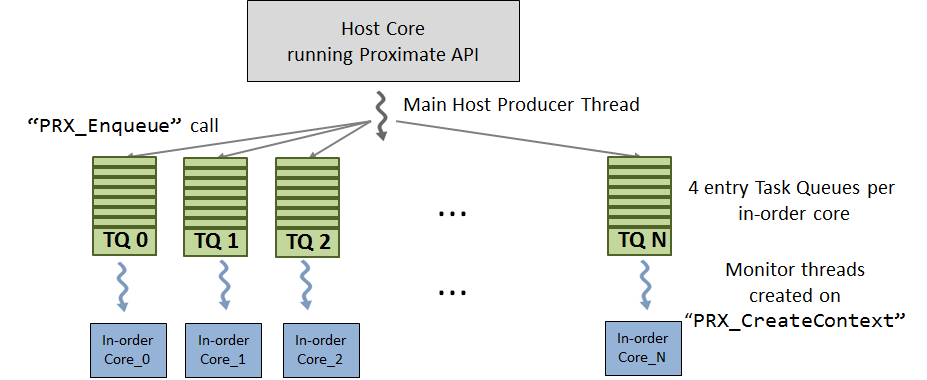
\includegraphics[width=0.9\linewidth, height=2.5in]{cs758-figs/q-model.png}
  \end{center}
\vspace{-0.2in}
  \caption{Proximate Task Based Queuing Model}
  \label{fig:q-model}
\vspace{-0.05in}
\end{figure}

Figure~\ref{fig:q-model} shows the high-level overview of the
Proximate queuing model which is implemented in ZSim simulator.
In this task based model, each in-order core has a 4 entry task-queue (TQ)
able to store the offloaded tasks/kernels. When the runtime on host core
calls the \emph{PRX\_CreateContext} with the number of pthread instances to be launched, 
that manu \emph{monitor threads} are created for each in-order to monitor the per-core
task queue. These monitor threads are always running threads monitoring the task-queue for new work, 
and destroyed only when the \emph{PRX\_Free} API is called.

Everytime, the host core running the proximate runtime offloads a task
using, \emph{PRX\_Enqueue} the task is scheduled on one of the task-queues on a round-robin fashion.
And when the task-queue gets full, the task scheduler will notify the host core not to issue anymore
kernel calls. We do not have a sophisticate load balancer one would need when handling with many kernels, 
but we consider that as a part of future work. 


\section{Methodology} \label{sec:meth}

This section describes our evalauation methodology for evaluating proximate and running the
proximate parallel programs.

\subsection{Workloads}
We first describe the workloads we have targetted and then the methodlogy to 
evlauate them. Since, proximate is aimed at high performance and throughput
for both regular and irreguaar workloads, we have considered both class of workloads
and their parallel implementations. 

\paragraph{Regular Worklaods}
Regular worklaods are generally the high-performance computing applications
which have following properties: i) regular streaming memory access patterns,
ii) Computationally intensive and iii) ample amount of data-level parallelism.
We consider deep learning neural networks kernels similar to Diannao accelerator engine~\cite{diannao}
and the convolution based image processing workloads from Convolution Engine~\cite{convolution_engine}.
Some other micro-benchmarks for functional evalaution considered are: Ocean, summation and reduction, 
but we don't consider in our performance evalaution. 


\paragraph{Irregular Worklaods}
Irregular workloads generally have i) irregular memory access patterns
with low ILP, ii) Ver small computations and iii) Data dependent control. 
For such workloads, we consider the graph based workloads like histogram, 
shortest path and breadth-first-search. 


\subsection{Simualation Methodology} 
For proximate multi-core riscv inorder core simualtion, 
we consider a multi-core simualtor called ZSim~\cite{sanchez2013zsim}, which is a
fast x86-65 simulator. It is based on dynamic binary translation and PIN~\cite{pin} model which natively 
runs the pthread instances of the kernel on the real hardware.  

\begin{figure}
  \begin{center}
    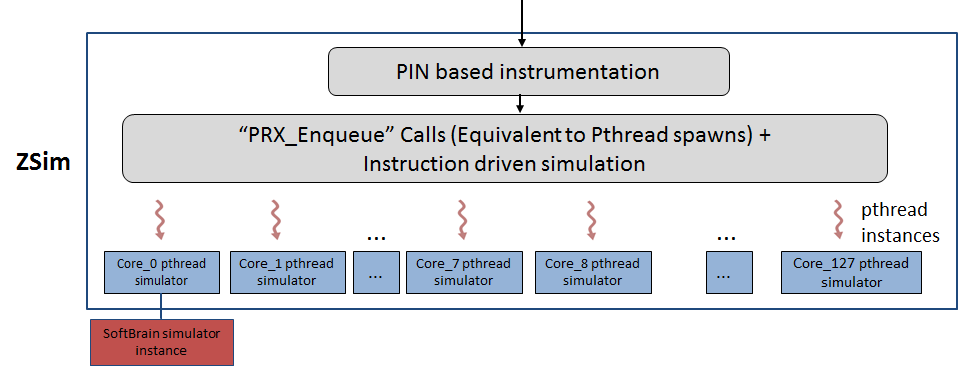
\includegraphics[width=\linewidth]{cs758-figs/zsim-meth.png}
  \end{center}
\vspace{-0.2in}
  \caption{ZSim based Proximate Simualtion}
  \label{fig:sim}
\vspace{-0.05in}
\end{figure}

Figure~\ref{fig:sim} shows our simulation methology, and  each compiled
proximate API based pthread program ins instrumented for multi-core simualtion initially.
Then, the proximate API based hooks would identify the proximate kernel and whenever ZSim main thread
encounters a \emph{PRX\_Enqueue} API call, it would offload the kernel to 
a) multiple in-order core pthread instances - if the kernel is an irregular type,  or b) Softbrain simualtor instance
which runs the softbrain portion of the kernel, if the kernel is a regualr type. 
Currenly, we don't have simualtor support to run, multiple instances of Softbrain kernels, 
and hence all the softbrain based parallel kernels need to be serialized to the same softbrain
simualtor instance. We aim to support this in our infrastructre in coming days. 


\begin{table}[]
  \centering
  \begin{tabular}{|l|l|}
    \hline
    \textbf{Baseline Configuiration} & \textbf{Explanation}                                \\ \hline
    \textit{pthread\_xeon}  & Pthread program run on a 64-core Xeon-Phi processor \\ \hline
    \textit{omp\_xeon}      & OpenMP program run on a 64-core Xeon-Phi processor  \\ \hline
  \end{tabular}
  \caption{Baseline Xeon-Phi configurations used for comaprison}
  \label{tab:base-config}
\end{table}

\subsection{Proximate Configurations}
In this section, we explain different configurations of proximate we have simulated, 
to compare agianst the real hardware. 

For comaprison of parallel program execution on proximate with
a server class processor, we first the baseline versions of parallel programs implemented in pthreads and OpenMP
running on r a 64-core 4way SMT Xeon-Phi processor.
Table~\ref{tab:base-config} explains the 2 baseline versions of parallel programs we run on Xeon-Phi machine.
We vary the number of threads for these 2 baselines, to find out the best design space w.r.t number of threads
and choose that as the comaprison point for proximate parallel program.

We now explain, the actual Proximate configurations simualted using the methodogy explained above. 
As we kno that current proximate hardware has \emph{1 host-core + 128 in-order cores + 1 Softbrain}, we try
to support the same hardware configuration in our simualtions. Although, ideally you would be needing 8 Softbrain 
instances runnign on each vault, our infrastrucure cannot support that for now and hence only 1 softbrain.

Based on kernel type, each proximate program can be simualted only on in-order cores without the quequing model
explained previoulsy here in Section~\ref{sec:queue}. Or, if more kernel instances are present in the program, then they 
can be dynamically spawned on the queuing model of proximate. When you have softbrain portions in the program, 
you would want to run on softbrain only simualtion. So, there are different ways of simuating proximate based on the kernel
type and Table~\ref{tab:real-configs} sumamrize the possible simaulted conifgurations for proximate. We would be using these
configurations for comparison in our evlaution. 


\begin{table}[]
  \centering
  \begin{tabular}{|l|l|}
    \hline
    \textbf{Proximate Configuration}               & \textbf{Explanation}                                                    \\ \hline
    \textit{prx\_inorder}                          & Proximate API pthread program w/o queuing model                         \\ \hline
    \textit{prx\_inorder\_q}                       & Proximate API pthread program with queuing model                        \\ \hline
    \textit{prx\_sb\_only}                         & Proximate API + single SoftBrain ‘only’ program                         \\ \hline
    {\color[HTML]{FE0000} \textit{prx\_multi\_sb}} & {\color[HTML]{FE0000} Proximate API + multi-threaded SoftBrain program -- Not simualted} \\ \hline
  \end{tabular}
  \caption{Proximate Simualted Configurations}
\label{tab"real-configs}
\end{table}

\section{Evaluatuion and Results} \label{sec:eval}

We first explain the workload progress state for each, and 
show what has been successfuly simulated w.r.t thier design space. 





%\input{summary}
\section{Challenges} \label{sec:chal}
The challenges we faced is implementing a queueing model on Zsim. 
The queueing model should mimic the Swarm style execution model 
to schedule and execute multiple irregular workloads concurrently. 
The challenge was debugging and getting to working in a short amount of time. 

Another challenge we faced is choosing the right base line for all 
experiments. Small workloads results in slowdown for pthreads and 
OpenMP while large workloads requires unaffordably slow runtimes on simulators. 
Furthermore, there were differences between real hardware and Zsim, 
each of which shows peak speedup at different kernel size or different number of threads. 
Therefore, we had to run preliminary results to get a estimate of which workload 
configurations works well on which parallel programming paradigms.

Yet another challenge that we faced is the large design space of 
programming paradigms for a large set of workload. The programming 
paradigms includes sequential, OpenMP, pthreads, proximate\_inorder, 
proximate\_inorder\_with\_queueing, proximate\_softbrain\_only. The workload suites include
neural networks DianNao, image processing convolution engine, and 
irregular graph workloads, each of which has multiple benchmarks. 

\section{Conclusion and Future Work} \label{sec:conc}
This project focused on exploring the parallel programming design space
of Proximate, a multi-tile programmable hardware accelerator.
The aim is to investigate the programming interface  of Proximate, the parallel
hardware improvements and in general explore the parallel programs run on proximate.
We have tried to explore a new type of the multi-tile programmable architecture,
its scalability and speedup of such accelerator architecture 
compared to a traditional server class multi-core processors for parallel programs.
In summary, we explored different programming design points in the project and proximate is able to achieve speedups of
50-100x over a traditional server class multi-core processor. 

Proximate is a programmable accelerator that targets high 
efficiency and programmability. It is a compute engine 
for both regular and irregular workloads.

Proximate exposes a flexible  programming model with a task-based programming API. 
The programmer manages data sharding to achieve task and data locality for performance and scalability. 
The simple queueing model supports more concurrency with locality 
as each worker thread will only execute tasks in their own queue. 
Preliminary results shows that Proximate outperforms current 
multiprocessor programming paradigms by a factor of 10x for regular 
workloads and a factor of 2x for irregular workloads. Although
multi-threaded SoftBrain may cause new issues such as synchronization, 
schedule, and saturate memory bandwidth, it could uncover new bounds of performance. We leave multi-threaded SoftBrain to future work. 



\section{Appendix}\label{sec:appendix}

This section acts as an appendix and explain an example Classifier program in Proximate space.  

\begin{figure}[h]
  \begin{center}
    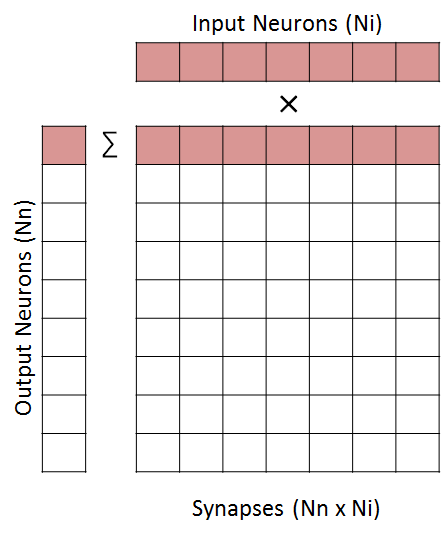
\includegraphics[width=0.3\linewidth]{cs758-figs/classifier-diagram.png}
  \end{center}
\vspace{-0.2in}
  \caption{Classifier workload diagram}
  \label{fig:classifier-diagram}
\vspace{-0.05in}
\end{figure}

Figure~\ref{fig:classifier-diagram} shows the classifier workload. 
Classifier requires multiplying the input neurons (a vector) by synapses 
(a matrix) and then doing the summation reduction.


\begin{figure}
  \begin{center}
    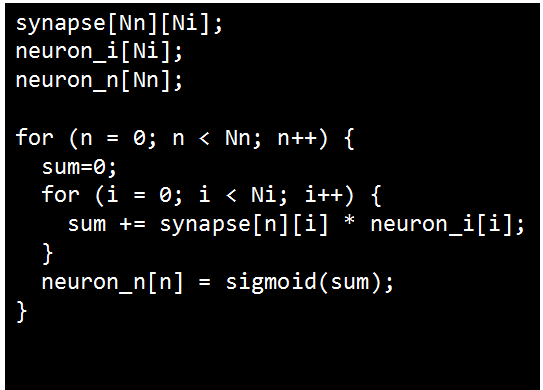
\includegraphics[width=0.5\linewidth]{cs758-figs/classifier-cpu.png}
  \end{center}
\vspace{-0.2in}
  \caption{Classifier implementation using sequential CPU}
  \label{fig:classifier-cpu}
\vspace{-0.05in}
\end{figure}

Figure~\ref{fig:classifier-cpu} shows the sequential implementation of 
classifier. Classifier can be done with a nested for loop to take the 
summation of the product between the input neurons and synapses.


\begin{figure}[h]
  \begin{center}
    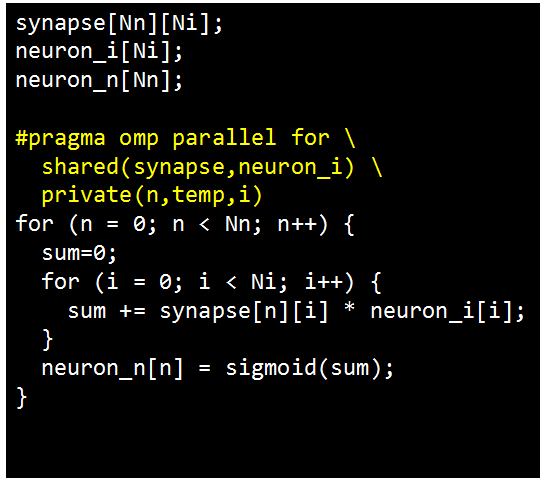
\includegraphics[width=0.5\linewidth]{cs758-figs/classifier-omp.png}
  \end{center}
\vspace{-0.2in}
  \caption{Classifier implementation using OpenMP}
  \label{fig:classifier-omp}
\vspace{-0.05in}
\end{figure}

Figure~\ref{fig:classifier-omp} shows the OpenMP implementation of 
classifier. The OpenMP implementation of classifier is using a 
\emph{\#pragma omp parallel} on the outer loop. 


\begin{figure}[h]
  \begin{center}
    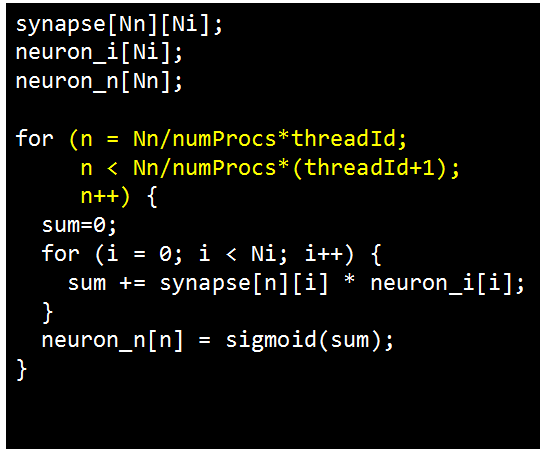
\includegraphics[width=0.5\linewidth]{cs758-figs/classifier-pthread.png}
  \end{center}
\vspace{-0.2in}
  \caption{Classifier implementation using pthreads}
  \label{fig:classifier-pthread}
\vspace{-0.05in}
\end{figure}

\paragraph{}

Figure~\ref{fig:classifier-pthread} shows the pthread implementation of 
classifier. The pthreads implementation of classifier shards the 
workload among pthreads. 


\begin{figure}
  \begin{center}
    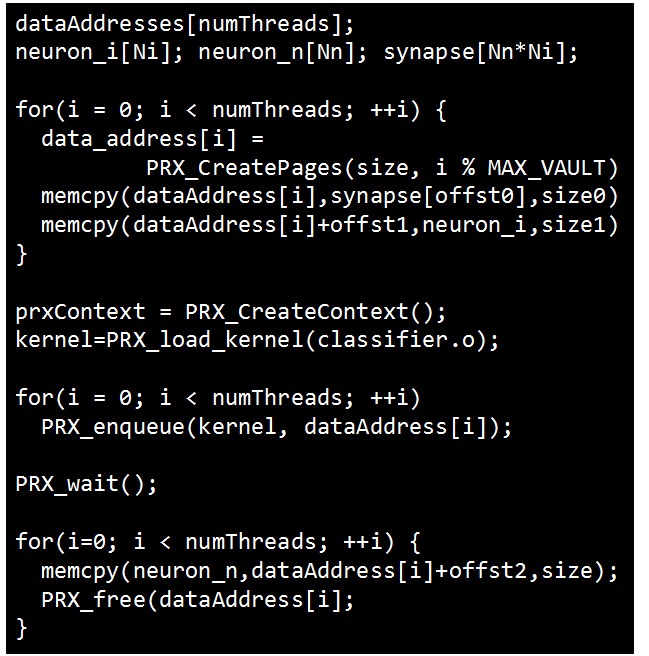
\includegraphics[width=0.5\linewidth]{cs758-figs/classifier-prx_inorder_q.png}
  \end{center}
\vspace{-0.2in}
  \caption{Classifier implementation using proximate with inorder cores and queuing model}
  \label{fig:classifier-prx_inorder_q}
\vspace{-0.05in}
\end{figure}

Figure~\ref{fig:classifier-prx_inorder_q} shows the proximate implementation 
with inorder cores and queuing model of classifier. The proximate queuing 
implementation of classifier shards the 
workload to different vaults. Calling create context 
will spawn threads to monitor work queues. Then, load the kernel so that each thread
know which kernel to execute upon receiving their thread arguments. 
Next, enqueue the workloads and wait for them to finish. 
Finally, gather the results back into a single array. 


\begin{figure}
  \begin{center}
    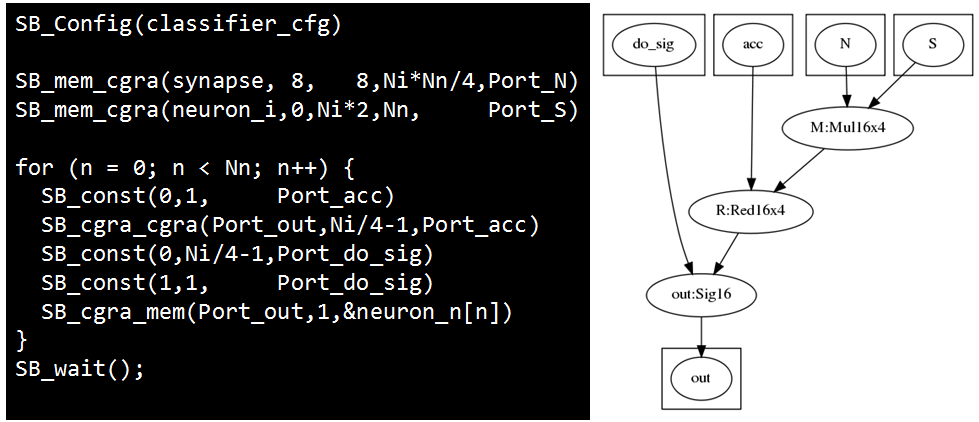
\includegraphics[width=\linewidth]{cs758-figs/classifier-prx_sb_only.png}
  \end{center}
\vspace{-0.2in}
  \caption{Classifier implementation using proximate with softbrain only}
  \label{fig:classifier-prx_sb_only}
\vspace{-0.05in}
\end{figure}

Figure~\ref{fig:classifier-prx_sb_only} shows the proximate implementation 
with softbrain only of classifier. The softbrain implementation first configures the
hardware to handle classifier. Then, pass inputs and synapses into softbrain. 
Loop through the softbrain fabric to do multiple iterations of the computation, one for each output.
Finally, wait for the softbrain computational fabric to finish. 


\singlespace
\bibliographystyle{abbrv}
\bibliography{prelim}

\end{document}
